% Name: Quadratic equation solver
% Description: Solving ax^2 + bx + c = 0 by the sign of the discriminant, with a branch for two real roots, one repeated root, and complex roots.
% Tags: flowchart, quadratic equation, discriminant, algorithm

\usetikzlibrary{shapes.geometric, shapes.misc, arrows.meta, positioning}

\begin{tikzpicture}[
  node distance=6mm and 10mm,
  every node/.style={font=\small},
  terminal/.style={rounded rectangle, draw, minimum width=18mm, minimum height=7mm},
  process/.style={rectangle, draw, minimum height=8mm, inner xsep=3mm},
  io/.style={trapezium, trapezium stretches body, trapezium left angle=70, trapezium right angle=110, draw, minimum height=7mm},
  decision/.style={diamond, aspect=2.2, draw, inner sep=1pt},
  arrow/.style={-{Stealth}, thick},
]
  \node[terminal] (start) {Start};
  \node[io, below=of start] (read) {Read $a \ne 0$, $b$, $c$};
  \node[process, below=of read] (disc) {$D \gets b^2 - 4ac$};
  \node[decision, below=of disc] (pos) {$D > 0$?};
  \node[decision, below=of pos] (zero) {$D = 0$?};
  \node[process, below=of zero] (cplx) {$x \gets \dfrac{-b \pm i\sqrt{-D}}{2a}$};
  \node[process, right=of pos] (two) {$x \gets \dfrac{-b \pm \sqrt{D}}{2a}$};
  \node[process, right=of zero] (one) {$x \gets -\dfrac{b}{2a}$};
  \node[io, below=of cplx] (print) {Print $x$};
  \node[terminal, below=of print] (stop) {Stop};
  \coordinate (bus) at ([xshift=6mm]two.east);

  \draw[arrow] (start) -- (read);
  \draw[arrow] (read) -- (disc);
  \draw[arrow] (disc) -- (pos);
  \draw[arrow] (pos) -- node[above] {yes} (two);
  \draw[arrow] (pos) -- node[right] {no} (zero);
  \draw[arrow] (zero) -- node[above] {yes} (one);
  \draw[arrow] (zero) -- node[right] {no} (cplx);
  \draw[arrow] (cplx) -- (print);
  \draw[arrow] (print) -- (stop);
  \draw[arrow] (two.east) -- (bus) |- (print.east);
  \draw[thick] (one.east) -- (one.east -| bus);
  \fill (one.east -| bus) circle (1.5pt);
\end{tikzpicture}
